\documentclass{article}

\usepackage[provide=*, magyar]{babel}

\usepackage{graphicx}
\usepackage{tikz}
\usetikzlibrary{calc}
\usepackage{calc}

\usepackage{pdfpages}

\usepackage{amsmath}
\usepackage{siunitx}
\usepackage{tabularx}
\usepackage{booktabs}
\usepackage[table]{xcolor}
\usepackage{multicol}

\newcommand{\siunit}[2]{
	\SI{#1}{[#2]}
}

\newcommand{\n}[1]{
	\siunit{#1}{\newton}
}
\newcommand{\nmm}[1]{
	\siunit{#1}{\newton\mm}
}
\newcommand{\kn}[1]{
	\siunit{#1}{\kilo\newton}
}
\newcommand{\knm}[1]{
	\siunit{#1}{\kilo\newton\meter}
}
\newcommand{\mpa}[1]{
	\siunit{#1}{\mega\pascal}
}

\newcommand{\equal}[2]{
	\sum{#1} := 0 = #2
}

\newcommand{\circled}[1]{
	\raisebox{.5pt}{\textcircled{\raisebox{-.9pt} {#1}}}
}

\title{Szilárdságtan HF1}
\date{\today}
\author{Vári Gergő}


\begin{document}
	\pagenumbering{gobble}
	
	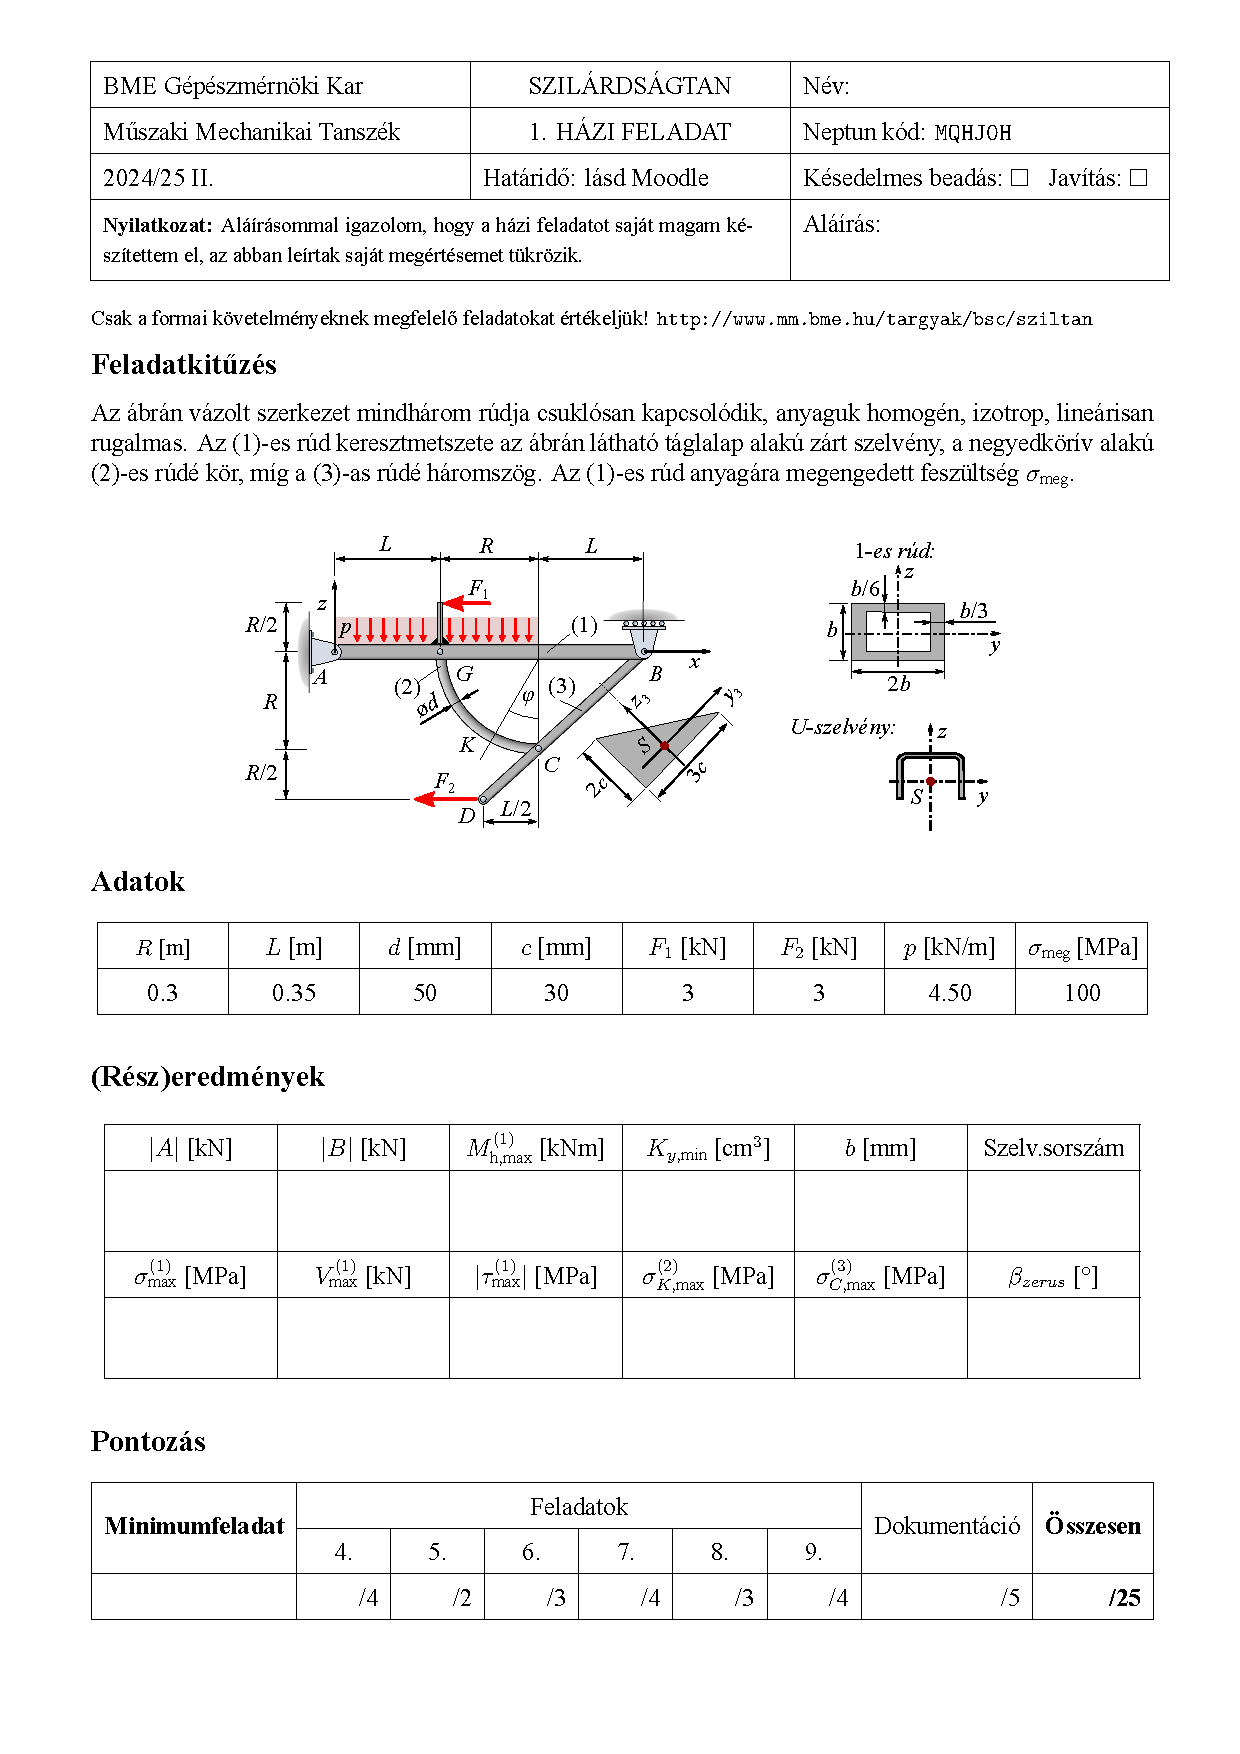
\includepdf[pages={1}, pagecommand={
	\begin{picture}(0,0) 
		\put(270, 93){Vári Gergő}
		{\fontfamily{cmr}\selectfont\put(300, 25){\Large{Vári Gergő}}}
		\put(-46, -417){\Large{6.1}}
		\put(29, -417){\Large{1.85}}
		\put(108, -417){\Large{0.35}}
		\put(189, -417){\Large{3.5}}
		\put(269, -417){\Large{24}}
		\put(344, -417){\Large{166}}
		\put(332, -475){\Large{-18.435}}
		\put(256, -475){\Large{33.333}}
		\put(176, -475){\Large{-21.331}}
		\put(111, -475){\Large{5.4}}
		\put(25, -475){\Large{1.576}}
		\put(-57, -475){\Large{-94.66}}
	\end{picture}
}]{szilhf1.pdf}


	\maketitle
	\rule{0pt}{50pt}
	\begin{figure}[hbt!]
		\centering
		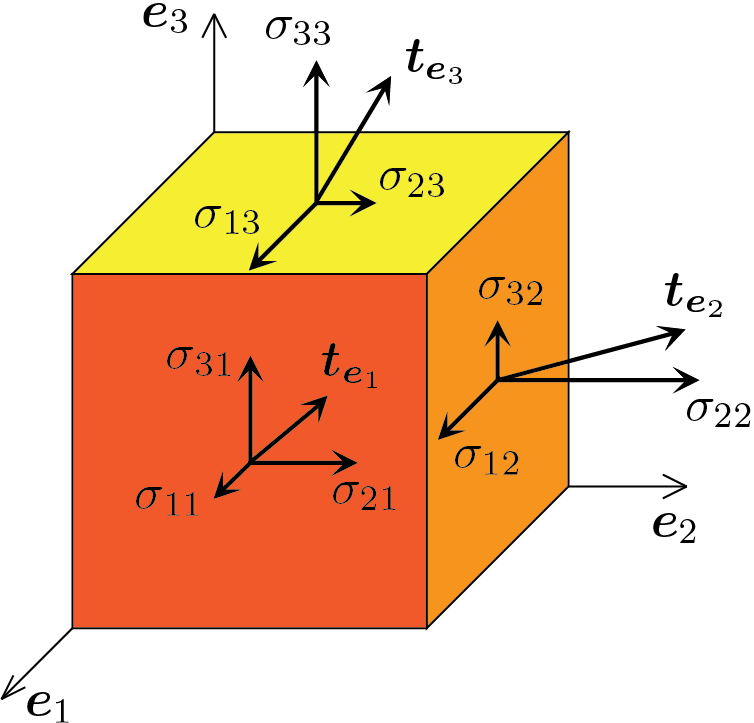
\includegraphics[scale=1.75]{./images/cauchy_stress_components.png}
		\caption{Cauchy feszültségi tenzor}
	\end{figure}

	\newpage
	\pagenumbering{arabic}
	
	\section{Reakció komponensek}

\subsection{Léptékhelyes ábra}

\begin{tikzpicture}
\end{tikzpicture}

\subsection{SZTÁ}

\newpage

\subsection{Egyensúlyi képletek}

\begin{align*}
	&\equal{F_x}{A_x - F_1 - F_2} \\
	&\equal{F_y}{A_y + B_y - p(L+R)} \\
	&\equal{M^A}
	{B_y(2L+R) + F_1 \frac{R}{2} - F_2 \left(R+\frac{R}{2}\right) - p\frac{(L+R)^2}{2}}
\end{align*}

\begin{align*}
	&A_x = F_1 + F_2 = \kn{6} \\
	&B_y 
		= F_2 \left(R + \frac{R}{2}\right) - F_1\frac{R}{2} + p\frac{(L+R)^2}{2} 
		= \kn{1.85} \\
	&A_y = p(L+R) - B_y = \kn{1.074} \\
\end{align*}

\begin{align*}
	&|\textbf{A}| = \kn{6.1} \\
	&|\textbf{B}| = \kn{1.85} 
\end{align*}

	\newpage

	\section{Csuklók és rudak}

\subsection{}

\subsubsection{SZTÁ}

\subsubsection{Egyensúlyi képletek}
\begin{align}
    &\equal{F_x}{A_x - F_1 + N_{2_x} + N_{1_x}} \\
    &\equal{F_y}{A_y - p(L+R) - N_{2_y} - N_{1_Y}} \\
    &\equal{M^B}{N_{2_y}(L+R) + F_1 \frac{R}{2} + p(L+R)(L+\frac{L+R}{2}) \nonumber \\
    &\quad - A_y (2L+R)}
\end{align}

\begin{equation}
	(5) \Rightarrow N_{2_y} = \frac{A_y{2L+R} - F_1 \frac{R}{2} - p(L+R)(L+\frac{L+R}{2})}{L+R} = \kn{-2.0775}
\end{equation}

\newpage

\subsection{}

\subsubsection{SZTÁ}

\subsubsection{Egyensúlyi képletek}
\begin{align}
    &\equal{F_x}{- N_{2_x} + N_{2_x}} \\
    &\equal{F_y}{- N_{2_y} + N_{2_y}} \\
    &\equal{M}{0}
\end{align}

\newpage

\subsection{}
\subsubsection{SZTÁ}
\subsubsection{Egyensúlyi képletek}
\begin{align}
    &\equal{F_x}{- F_2 + N_{3_x} - N_{2_x}} \\
    &\equal{F_y}{N_{2_y} + N_{3_y}} \\
    &\equal{M^C}{-F_2 \frac{R}{2} - N_{3_x} (R) + N_{3_y} (L)}
\end{align}

\newpage

\subsection{B pont}

\subsubsection{SZTÁ}

\subsubsection{Egyensúlyi képletek}
\begin{align}
    &\equal{F_x}{-N_{1_x} + N_{3_x}} \\
    &\equal{F_y}{N_{1_y} + B_y - N_{3_y}} \\
\end{align}

\newpage

\subsection{Összegzés}
\begin{align*}
	N_1 &= &\begin{bmatrix}
		0.92375 \\
		0.2265
	\end{bmatrix} \kn{}\\
	N_2 &= &\begin{bmatrix}
		-2.0775 \\
		-2.0775
	\end{bmatrix} \kn{}\\
	N_3 &= &\begin{bmatrix}
		0.92375 \\
		2.0775
	\end{bmatrix} \kn{}\\
\end{align*}

	\newpage

	\section{1-es rúd igénybevételei}
\subsection{SZTÁ}

\newpage

\subsection{Függvények}
{\footnotesize
	\begin{center}
		\setlength{\aboverulesep}{0pt}
		\setlength{\belowrulesep}{0pt}
		\setlength{\extrarowheight}{.75ex}
		\begin{tabular}{rccc}
			\toprule
			\rowcolor{lightgray}
			$x$
			&$0 < x < L$
			&$L < x < L+R$
			&$L+R < x < 2L+R$ \\

			\toprule

			\rowcolor{pink}
			$N$
			&$-A_x$
			&$-A_x - N_{2_x} + F_1$
			&$-A_x - N_{2_x} + F_1$ \\

			\midrule

			\rowcolor{lime}
			$V$
			&$-A_y+px$
			&$px -A_y + N_{2_y}$
			&$p(L+R) - A_y + N_{2_y}$ \\

			\midrule

			\rowcolor{cyan}
			$M_h$
			&$
			-A_y x + p \frac{x^2}{2}
			$
			&$
			\begin{array}{c}
				-A_y x + p \frac{x^2}{2} \\
				+ N_{2_y}(x - L) + F_1 \frac{R}{2}
			\end{array}
			$
			&$
			\begin{array}{c}
				\\
				-A_y x + p (L+R) \left( L-\frac{L+R}{2} \right) \\
				+ N_{2_y}(x - L) + F_1 \frac{R}{2} \\
				\\
			\end{array}$ \\

			\bottomrule
		\end{tabular}
	\end{center}
}

\newpage

\subsection{Ábrázolás}

	\newpage
	
	\section{Méretezés}

\subsection{Veszélyes keresztmetszet}

\subsection{Keresztmetszeti tényező}

	\section{Helyettesítés U-szelvénnyel}


	\section{U-szelvény ellenőrzése normálerő hatására}

\subsection{Ellenőrzés}

\subsection{Normálerő ábrázolása}

\subsection{Maximális feszültség}

	\newpage

	\section{Nyírásból adódó csúsztató feszültség}

\subsection{Függvény}

\subsection{Ábrázolás}

	\newpage

	\section{2-es rúd igénybevételei}

\subsection{SZTÁ}

\newpage

\subsection{Függvények}

\begin{equation*}
	\phi = \ang{30}
\end{equation*}

\begin{align*}
	N(\phi) 
	&= N_{2_x} \cdot \cos\phi + N_{2_y} \cdot \cos\left(\ang{90}-\phi\right) \\
	&= N_{2_x} \cdot \cos\phi + N_{2_y} \cdot \sin\phi \\
	N(\ang{30}) &= \n{-2837.92}
\end{align*}

\begin{align*}
	V(\phi) &= -N_{2_x} \cdot \sin\phi + N_{2_y} \cdot \sin\phi \\
	V(\ang{30}) &= \n{-760.42}
\end{align*}

\begin{align*}
	M_h(\phi) &= N_{2_x} \cdot R \left(1 - \cos\phi\right) - N_{2_y} \cdot R\sin\phi \\
	M_h(\ang{30}) &= \nmm{228125.3329}
\end{align*}

\newpage

\subsection{Normálfeszültség ábrázolása}

\subsection{Maximális normálfeszültség}

\begin{align*}
	\frac{R}{d} = 6 \Rightarrow \sigma(y) &= \frac{N}{A} + \frac{M_h}{R\cdot A} + \frac{M_h}{I_x} \cdot \frac{R\cdot y}{R+y} \\
	A &= \frac{d^2 \pi}{4} = 625\pi \\
	I_x &= \frac{d^4 \pi}{64} = \frac{390625}{4}\pi
\end{align*}

\begin{align*}
	\sigma(\frac{d}{2}) &= \mpa{16.1} \\
	\sigma(0) &= \mpa{-1.058} \\
	\sigma(-\frac{d}{2}) &= \mpa{-21.34}
\end{align*}

	\newpage
	
	\section{3-as rúd hajlítása}

\begin{equation*}
	c = \siunit{30}{\mm}
\end{equation*}

\subsection{Zérus és $y_3$ tengely szöge}
A főfeszültségekből kitudjuk számolni a keresett szöget.
\begin{align*}
	&I_{x_3} = \frac{(3c)(2c)^3}{36} = &\siunit{5.4e5}{\mm^4} \\
	&I_{y_3} = \frac{(2c)(3c)^3}{36} = &\siunit{1.215e6}{mm^4}\\
	&I_{xy_3} = \frac{(2c)^2(3c)^2}{72} = &\siunit{-4.05e5}{mm^4}
\end{align*}

\begin{align*}
	I_{1;2} &= \frac{I_{x_3} + I_{y_3}}{2} + \frac{1}{2}\sqrt{(I_{x_3} - I_{y_3})^2 +4I_{xy_3}^2} \\
	I_1 &= \siunit{1404691,853}{\mm^4} \\
	I_2 &= \siunit{350308.1469}{\mm^4}
\end{align*}

\begin{equation*}
	\alpha = \arctan\left(\frac{I_{x_3} - I_1}{I_{xy_3}}\right) = \ang{64.9}
\end{equation*}

\begin{align*}
	M_h &= - F_2 \frac{R}{2} = &\knm{-0.45} \\
	M_{h_\xi} &= \left|M_h\right|\cdot \cos\alpha = &\nmm{190889.7402} \\
	M_{h_\eta} &= \left|M_h\right|\cdot \sin\alpha = &\nmm{-407505.9596} \\
\end{align*}

\begin{align*}
	\beta &= \arctan\left(\frac{M_{h_\eta}\cdot I_1}{M_{h_\xi}\cdot I_2}\right) = &\ang{-83.3367} \\
	\beta_0 &= \alpha + \beta = &\ang{-18.437}
\end{align*}

\subsection{Maximális normálfeszültség}

\begin{align*}
	\xi(x;y) &= x\cdot \cos\alpha + y\cdot \sin\alpha \\
	\eta(x;y) &= y\cdot \cos\alpha - x\cdot \sin\alpha \\
\end{align*}

\begin{equation*}
	\sigma(x;y) = \frac{M_{h_\xi}}{I_1}\eta(x;y) - \frac{M_{h_\eta}}{I_2}\xi(x;y)
\end{equation*}

\begin{align*}
	\sigma_A &= \sigma\left(-c;\frac{4}{3}c\right) = &\mpa{33,331} \\
	\sigma_B &= \sigma\left(-c;-\frac{2}{3}c\right) = &\mpa{-33,334} \\
	\sigma_C &= \sigma\left(2c;-\frac{2}{3}c\right) = &\mpa{2.52080429e-3}
\end{align*}

\begin{equation*}
	\sigma^{(3)}_\text{C,max} = \sigma_B = \mpa{-33.334}
\end{equation*}

\end{document}
